\documentclass[12pt,a4paper]{report}
\usepackage[textsize=tiny,
	% disable,
	]{todonotes}

 \newcommand{\ramon}[2][]{\todo[color={green!20},linecolor={green!100},#1,size=\tiny]{Ramon: #2}}

% Packages:
% \usepackage{listings}
\usepackage{environ}
\usepackage[utf8]{inputenc}
\usepackage[english]{babel}
\usepackage{fancybox}
\usepackage{float}
\usepackage{algorithm}
\usepackage{algpseudocode}
\usepackage[margin=2.5cm]{geometry}
\usepackage{graphicx} 
\usepackage{gensymb}
\usepackage{amsmath}
\usepackage{fancyvrb}
\usepackage{tikzit}
\usepackage{pgfplots}
% \usepackage{mathptmx}
\begin{tikzpicture}
	\begin{pgfonlayer}{nodelayer}
		\node [style=Box] (0) at (-9.5, 0) {Environment};
		\node [style=Box] (1) at (0, 0) {Problem Generator};
		\node [style=Box] (2) at (8.5, 0) {Planner};
		\node [style=Box] (3) at (-4, 4) {Domain};
		\node [style=none] (6) at (3.5, 0) {};
		\node [style=none] (7) at (6.5, 0) {};
		\node [style=none] (8) at (-2, 3) {};
		\node [style=none] (9) at (0, 1) {};
		\node [style=none] (10) at (-7, 0) {};
		\node [style=none] (11) at (-3.75, 0) {};
		\node [style=none] (12) at (10.5, 0) {};
		\node [style=none] (13) at (13.5, 0) {};
		\node [style=Box] (15) at (15.5, 0) {Plan};
		\node [style=none] (17) at (5, 0.5) {$\mathcal{P}$};
		\node [style=none] (18) at (-8.75, 1) {};
		\node [style=none] (19) at (-6, 3) {};
	\end{pgfonlayer}
	\begin{pgfonlayer}{edgelayer}
		\draw [style=Arrow] (10.center) to (11.center);
		\draw [style=Arrow] (8.center) to (9.center);
		\draw [style=Arrow] (6.center) to (7.center);
		\draw [style=Arrow] (12.center) to (13.center);
		\draw [style=Arrow] (18.center) to (19.center);
	\end{pgfonlayer}
\end{tikzpicture}

\input{directional.tikzstyles}

% Colors:
% \usepackage[dvipsnames]{xcolor}
% \definecolor{backcolour}{rgb}{0.95,0.95,0.92}

% PDDL code style:
% \lstdefinestyle{PDDL}{
%     % backgroundcolor=\color{backcolour},
%     basicstyle=\ttfamily\footnotesize\bfseries,
%     breakatwhitespace=false,         
%     breaklines=true,                 
%     captionpos=t,                    
%     keepspaces=true,                 
%     numbers=left,                    
%     numbersep=5pt,                  
%     showspaces=false,                
%     showstringspaces=false,
%     showtabs=false,                  
%     tabsize=2
% }
% \lstset{
%     style=PDDL, 
%     frame=shadowbox,
%     rulesepcolor=\color{black},
% }

% Defs:
\mathchardef\mhyphen="2D




\begin{document}

\begin{titlepage}
    \begin{center}
        \vspace*{1cm}

        \Huge
        \textbf{Solving Complex Path Finding Games with Generalised Planning}
            
        \vspace{0.5cm}
        \LARGE
        Supervised by Ramon Fraga Pereira
            
        \vspace{1.5cm}
            
        \textbf{Murtaza Daudali}
            
        \vfill
            
        A report submitted  for the degree of \\Bachelor of Science
            
        \vspace{0.8cm}
            
        \includegraphics[width=0.4\textwidth]{logo.jpeg}
            
        \Large
        Faculty of Science and Engineering\\
        University of Manchester\\
        2023-24
            
    \end{center}
\end{titlepage}

\setcounter{tocdepth}{1}
\tableofcontents
\listoffigures
\listoftables

\chapter*{Declaration}
I declare that this report is my own original work and has not been submitted for any assessment or award at University of Manchester or any other university and that no portion of the work referred to in the report has been submitted in support of an application for another degree or qualification of this or any other university or other institute of learning.

\chapter*{Abstract}
Path finding, a fundamental aspect of gaming and Artificial Intelligence (AI), has garnered significant attention in recent years. This report delves into the complexities of path finding, exploring its applications in gaming. While traditional AI planning has focused on solvable instances, the emergence of generalized planning presents new opportunities and challenges. This project aims to explore the implications of extracting more general solutions for \textit{complex path finding} problems. Motivated by the scarcity of tools leveraging generalized planning in gaming, this project seeks to develop a suite of complex path finding \textit{problem generators}. These problems generated by these generators are designed to push the boundaries of existing planners, fostering an environment for academic exploration and advancement. Targeted towards students and enthusiasts in Knowledge-Based AI, this report provides insights into both classical and generalized planning methodologies. The objectives of this project include exploring state-of-the-art planners, modeling path finding problems, creating intuitive visualizations, analysing planner performance, and comparing classical versus generalized plans. Through these objectives, the project aims to furnish an easy-to-use tool with optimized planning examples, facilitating learning and development in the domain of AI.

\chapter{Introduction}
\section{Motivation and Context}
Path finding in games is a topic that has been researched by many researchers in recent history. It is a complex problem that involves the use of a variety of algorithms. Techniques used in path finding are not limited to games, and can be used in a variety of fields within Artificial Intelligence (AI), such as robotics and logistics. Generalised planning is a relatively new field in AI, traditionally focusing on solvable instances in the synthesis of programs (2003)\cite{jimenez_review_2019} to uses in robotics seen since the previous decade. It involves complex theory to solve a collection of planning instances in a single algorithm-like plan. These problems share the same observations and actions from some real world \textit{environment}. Computing this algorithm gives the individual solutions to the given planning instances. Due to its novelty, this project aims to expand the horizons by utilising these planners in gaming notably simple path finding games, evaluating its performance and its limitations. \\\\
Another motivation behind this project is to develop a series of \textit{complex path finding problems} that test the limits of generalised planners developed in the recent years. This stems from the lack of existing tools that utilise generalised planning, as the focus is usually on \textit{classical planning}. These problems must developed in a way such that existing planners can solve these problems in the most efficient way possible. This project is aimed at students and anyone who are looking to further their knowledge in the field of Knowledge-Based AI. Although the primary focus of this project is generalised planning, as classical planning is relevant to the field, it is also covered widely within this report. 


\newpage
\section{Aims and Objectives}
Due to the complexities involved in generalised planning, the goal of this project is to provide a easy-to-use tool with optimised planning examples, that students can use, learn and also develop from. Initially, this project focused only on Maze games, however this was extended to evaluate a variety of path finding games. Below are the objectives that have been outlined before the development of this project:

\begin{table}[ht]
\centering
\begin{tabular}{|p{0.473\linewidth}|p{0.473\linewidth}|}
\hline
Objective & What it involves \\\hline
Explore state-of-the-art planners used in Automated Planning in recent years & This involves researching both classical planners and generalised planners. \\\hline
Model path finding problems (Maze and Snake) as planning problems & This involves first creating the path finding problem in some format, then converting it into some instance that can be solved using a planner.
\\\hline
Create easy-to-understand visuals that displays generated path finding problems & This also involves creating interactive displays in which the user can create solvable path finding problem instances. \\\hline
Perform analysis on the performance of generalised planning on the created path finding problem instances & This involves measuring the impact of the size of paths created, or other various variables induced on the creation of plans from path finding problem instances.
\\\hline
Compare the plans generated by classical plans and generalised plans & This involves an investigation that finds answers the question: \textit{in which situations does one planner perform better than the other?}
\\\hline
\end{tabular}
\caption{Aims and Objectives}
\end{table}

\section{Report Structure}
This report starts with a brief introduction involving the motivation behind this project as well as the objectives that must be met in the finished product. The \textbf{2. Background} section explores the technical knowledge required to understand the report fully. This will include the history of planning starting from knowledge-based agents, to modern generalised planning. Then in the \textbf{3. Design and Implementation} section, a description of the design used in the creation this project will be given, including the architecture and \textit{problem generators}. The \textbf{4. Experiments and Evaluation} section will cover a variety of experiments that test the applicability of planners on the create path finding instances. Finally the report will conclude with the \textbf{5. Summary and Conclusions} section that will critically analyse the project as a whole, as well as listing the achievements met by this project and any future work that could improve the final design.

\chapter{Background}
\section{Logical Agents}
Humans do things based of the process of reasoning that operate on internal representations of knowledge, in AI, reasoning is embodied in knowledge-based agents \cite[Chapter 7]{russell2016artificial}. When states are only partially observable, i.e, the agents information set is not trivial, the agent must explore all possibilities before moving. With the development of heuristics and the use of some knowledge-base, the agent can act with a sense of logic. This project focuses on knowledge-based agents without additional mechanisms that provide learning.\\

\noindent A well made knowledge-based agent can be designed by giving it a sequence of actions or procedures to follow, with a combination of statements telling the agent how to follow them. \cite[Chapter 7]{russell2016artificial} These are included within the agent's knowledge base. We can construct these sentences in propositional logic. A sentence is constructed from atomic sentences and complex sentences, where atomic sentences consist of a single proposition symbol i.e $\top$ (True), $\bot$ (False), $P$, $Q$, etc; and complex sentences are comprised of atomic sentences and connectives. For example, in a knowledge-base with two propositional letters $p$ and $q$, the 4 connectives to note \cite[Chapter 7]{russell2016artificial} used in this report are:

\begin{itemize}
    \item $\neg p$ (not p), $\neg$ flips the truth value of $p$
    \item $p \land q$ (p and q), $\land$ is the symbol for a conjunction, both $p$ and $q$ must be $\top$ for $p \land q$ to be $\top$ 
    \item $p \lor q$ (p or q), $\lor$ is the symbol for a disjunction, either $p$ or $q$ must be $\top$ for $p \lor q$ to be $\top$
    \item $p \rightarrow q$ (p or q), $\rightarrow$ represents an implication, it is usually read as: if $p$, then $q$. $p \rightarrow q$ is only $\bot$ if $p = \top$ and $q = \bot$ 
\end{itemize}

\noindent These propositional letters are used to define situations in the environment. For example, in the knowledge-base of an agent, $p_{x, y}$ would be $\top$ if the agent is at position $(1, 0)$ in the environment. The procedures and actions are used to set the truth value of these predicates. Further explanations of this are given in the following section.

\newpage
\subsection{Logical Inference and Plans}
After the construction of the agents knowledge-base $KB$, we want to determine whether the agent can arrive at some conclusion $\alpha$ in a finite number of steps. I.e. can the agent reach some goal state given $KB$? Formally this problem is written as $KB \models \alpha$. This has been proven to be decidable by the works of Godel and Turing \cite[Chapter 7]{russell2016artificial}. A plan is defined as a sequence of actions that lead to the solution of the goals set in an environment. These actions must declare what variables change and what stays the same in its definition \cite[Chapter 7]{russell2016artificial}.

\begin{itemize}
    \item The initial definition of states.
    \item The successor-state axioms for all possible actions at each time up to some maximum time $t$. In this report, we assume that an action takes up 1 unit of time.
    \item The assertion that the goal is achievable at time $t$, i.e $\alpha^t = \top$
\end{itemize}

\noindent After generating this sentence, if there exists some assignment of truth values to the variables in the sentence such that the sentence resolves to $\top$. We can extract those variables in the sentence that are assigned to $\top$. This represents a plan that achieves the goal $\alpha$. \cite[Chapter 7]{russell2016artificial} This truth assignment can be found through truth table look-ups or logical inference rules, that isn't covered in this report, however in problems with complex environments, this becomes significantly more computationally complex to compute. For example, using propositional inference, generating a sentence to prove that the agent can reach all locations would involve observing every location, in every orientation available to the agent. When looking at situations where the agent must avoid locations or collect items, it can be seen that this would become very costly.

\section{Classical Planning}
Due to the limitations of these hybrid propositional logic agents on complex environments, classical planning was developed to devise a faster method of generating plans to reach a goal. The agent's $KB$ is instead modelled as a problem that consists of first-order-logic and action schema. \cite[Chapter 10]{russell2016artificial} Classical planning is the successor to STRIPS planning which used the notion of knowledge-based agents. \cite{suárezhernández2021strips}

\subsection{First-Order Logic}
Propositional logic focuses on the truth relation between sentences and possible worlds, which lacks the expressive capability to describe an environment with many objects. \cite[Chapter 8]{russell2016artificial} For example to write the statement: "the box is on the floor" is very difficult using propositional sentences. First-order-logic is built around more complex relationships between objects in an environment, instead of simply stating that whether or not something exists within the environment \cite[Chapter 8]{russell2016artificial}.

\subsubsection{Domains}
The domain of a first-order logic model is the set of objects or domain elements that it contains \cite[Chapter 8]{russell2016artificial}. In this report, we deal with non-empty domains, every environment must contain at least one thing that can be expressed or described. These objects may have some relation. For example, in an environment with a table and floor we could see the mappings: \[(table \rightarrow position), (floor \rightarrow position)\]

\subsubsection{Definitions (Predicates, Fluents, Objects and Quantifiers)}
In first-order logic, we write relations using predicate symbols. The example statement can be expressed in first-order logic as the predicate: $On(box, floor)$, where $On$ is the predicate symbol; $box$ and $floor$ are the objects. A predicate has a fixed number of arguments that returns either $\top$ or $\bot$. A fluent is a condition that can change over time, as we model actions that take up a constant unit of time, we define fluents as a statement containing a predicate and its truth value. For example, if in our environment the box is on the floor then a fluent in the agent's knowledge-base would be: $On(box, floor) = \top$. First-order logic statements can also be quantified, for example, to state that all objects $x$ in our domain are positions, we would write the expression: $\forall x, (x \rightarrow position)$.  $\forall$ means "for all" and $\exists$ means "there exists". \cite[Chapter 8]{russell2016artificial}

\subsection{Planning Domain Definition Language (PDDL)}
In response to the limitations imposed by propositional inference based agents, planning researchers, notably Drew McDermott developed a factored representation in which the state of an environment is represented by a collection of variables. This family of languages is called the Planning Domain Definition Language (PDDL). \cite{ghallab_pddl_1998} This report focuses on PDDL1.2 which focuses on a primarily predicate way of modelling. PDDL requires four things to define a state search problem, three of which are used in the generation of sentences in plan synthesis mentioned in the previous section. The requirement for successor-state axioms is split into two parts: the actions available within a state and the result of applying an action. A state is represented as a conjunction of fluents, for example if the box is on the floor and there is a bear on the table, we can model this as: $On(box, floor) \land On(bear, table)$. States cannot contain fluents that contain variables or functions, they must be ground \cite[Chapter 10]{russell2016artificial}, for example $At(x)$ is not allowed if $x$ can vary at that state.

\subsubsection{Action Schema}
In PDDL, actions are described by a set of action schema, each action contains a precondition and an effect. The precondition is a sentence that must return $\top$ before the effect is evaluated. The effect sets the given sentence to $\top$. For example, below is action schema that moves the tells the agent to move an object $object$ from position $from$ to position $to$ in first-order logic \cite[Chapter 10]{russell2016artificial}: 

\begin{align*}
    Acti&on(move(object, to, from),\\
        &\text{\textsc{Precondition:}}\: At(object, to) \land Path(to, from)\\
        &\text{\textsc{Effect:}}\: At(object, from))
\end{align*}
\newpage

\noindent In PDDL the $move(object, to, from)$ action is shown below in Figure 2.1:

\begin{figure}[h!]
\centering
\begin{BVerbatim}
(:action move
    :parameters (?object ?to ?from)
    :precondition (and (at ?object ?to) (path ?to ?from))
    :effect (and (at ?object ?from))
)
\end{BVerbatim}
\caption{PDDL Action Example}
\end{figure}

\noindent The precondition occurs at time $t$ and the effect occurs at time $t+1$. An action $a$ can be executed in some state $s$ if $s \models Precondition(a)$ \cite[Chapter 10]{russell2016artificial}. 

\subsubsection{Planning Domains and Problems}
The set of action schemas is defined within the planning domain, along with types, constants and available predicates in the knowledge-base. The planning problem contains the initial truth values of fluents from predicates in the domain; objects, and the goal state $\alpha$ \cite{ghallab_pddl_1998}. Examples of these are covered within the Design section of this report. To note: this report focuses on the agent having full state observability and the actions in the domain are all deterministic, i.e there the result of an action can be determined.

\subsubsection{Formalism}
In this report, a classical planning instance (known as a PDDL problem) is the quadruple $P = \langle X, A, I, G \rangle$. where \cite{segovia-aguas_generalized_2021}:
\begin{itemize}
    \item $X$ is the set of state variables, which is the set of all possible predicates. As mentioned previously a state is the conjunction of fluents, this can also be described as: $x \in X$ $s_t = \langle x_0 = v_0, ..., x_{|X|} = v_{|X|} \rangle$ where $v_k$ is the truth value assigned to the predicate $x_k$ and $s_t \in S$ is the state observed at time $t$. $X$ must be non-empty as it describes the environment defined within a problem.
    \item $A$ is the set of action schema
    \item $I$ is the initial state, $I \in S$ 
    \item $G$ is a goal condition on the state variables $X$ that induces a set of goal states $S_G$ that is a subset of $S$, $S_G = \{s \mid s \models G, s \in S\}$.
\end{itemize}

\noindent A plan $\pi = \langle a_1, ..., a_m \rangle, a_i \in A$ \textit{solves} $P$ if the execution of $\pi$ with $s_0 = I$ finishes in a goal state $s_m \in S_G$ for some $m \leq |S_G|$. The plan $\pi$ is \textit{optimal} if $|\pi|$ is minimal amongst the plans that solve the problem $P$. In this report, the \textit{cost} of generating $\pi$ is $|\pi|$ \cite{segovia-aguas_generalized_2021}.

\subsection{Fast Downward}
Fast Downward is a classical planning system, designed specifically for solving deterministic planning problems. It employs a forward heuristic search methodology \cite{heuristicplanning}, to navigate through the state space. This methodology yields low-cost plans that are efficienctly discovered \cite{helmert_fast_2006}.  Fast Downward is authored notably by Malte Helmert, and has received contributions from numerous researchers and developers over the years, maintaining its relevancy in modern classical planning. The planner is renowned for its performance and adaptability. Fast Downward utilizes heuristics to navigate through the state space. \cite{helmert_fast_2006}. In the 9th International Planning Competition (IPC), Fast Downward was utilized by two winning planners \cite{vie2022adversarial}. Its performance in the IPC shows its capability to find optimal or near-optimal plans within specified time constraints. Fast Downward serves as the classical planner used in the synthesis of all classical planning instances within this project.

\section{Generalised Planning}
Generalised planning is a shift in focus away from generating plans quickly, but instead focuses on the structure of the plan generated. Generalised planning attempts to synthesise a plan over a set of classical planning instances $\mathcal{P}$, where $|\mathcal{P}| \geq 1$. These instances are all problems that share the same domain. A generalised plan has an algorithm-like solution that is valid over $\mathcal{P}$. \cite{jimenez_review_2019} The algorithm produced can be in a variety of theories/languages. In this report, generalised solutions are produced in a C++ manner, utilising pointers and control flow structures \cite{segovia-aguas_representation_2022}. Furthermore, a generalised plan is a generative model, a top-down approach begins with an empty program of set length, and iteratively generates lines of the algorithm until a solution is found that solves all the planning instances \cite{jimenez_review_2019}. The generalised plan can then be used to generate the classical plans for each planning instance \cite{jimenez_review_2019}. Due to the nature of this task, generalised planning is computationally expensive, taking exponentially more time in the worst case than classical planning. The upper bound on the number of actions is given by the total number of possible states of the generalised plan \cite{backstrom_automaton_plans}. 

\subsection{Best First Search Generalised Planning (BFGP)}
Due to the complexity of generalised planning, researchers (Javier, Sergio, Angers) have developed methods to find generalised plans in a much more reasonable time frame through optimising classical planning, alongside the well-known Best First Search (BFS) algorithm \cite{segovia-aguas_generalized_2021}.

\subsubsection{Planning with Pointers}
The planning model is extended with the use of a memory unit that contains $|Z| + 2$ pointers. This allows for powerful memory management so that reusing defined state variables across $\mathcal{P}$ takes up less space in actual memory. The $Z$ pointers reference the original planning state variables, in the memory unit. The other two pointers are zero and carry bit flags. For a classical planning instance $P = \langle X, A, I, G \rangle$, the extended model with registers is defined by $P_Z =\langle X_Z', A_Z', I_Z', G \rangle$ where \cite{segovia-aguas_generalized_2021}:

\begin{itemize}
    \item $X_Z' = X \cup \{y_z, y_c\} \cup Z$, where $\{y_z, y_c\}$ are the respective flags and $Z$ is the non-empty set of pointers of length $|X|$.
    \item $A_Z' = A' \cup R_Z$, where $A'$ is the set of action schema $A$ that uses pointers as parameters instead of objects. The set $R_Z = \{inc(z1), dec(z1), cmp(z1, z2), cmp(\text{*} z1, \text{*} z2), \\set(z1, z2) \mid z1, z2 \in Z\}$ is the set of actions that modify some pointers $z1, z2 \in Z$. 
    \item $I_Z'$ is the same initial state as defined by $I$, with the addition of $y_z = \bot, y_c = \bot$
\end{itemize}

\noindent A generalised plan is defined by $\Pi = \langle a_1, ..., a_m, end \rangle,\, a_i \in A_Z$. $\Pi$ can contain $goto$ instructions that reference another program line in the program, and the final element of $\Pi$ is always $end$. $\Pi$ solves $\mathcal{P}$ if there execution of all plans $\pi_i, (1 \leq 0 \leq |P|) $ generated by the algorithm described in $\Pi$ solves $P_i \in \mathcal{P}$. The \textit{cost} of $\Pi$, given by the sum of the length of the classical plans. The emprical performance measure is important within experiments in this report when we look at the FastDownward's plan synthesis in comparison to the solutions generated by BFGP \cite{segovia-aguas_generalized_2021}.

\subsubsection{Evaluation and Heuristics}
The evaluation is taken over a set of functions $f(\Pi)$ where $\Pi$ is a \textit{partially specified} generalised plan. In this report, a partially specified generalised plan is an incomplete generalised plan where the the full algorithm that solves all the planning instances has not been generated fully. This evaluation score yields stronger positive values as it $\Pi$ gets closer to solving all problems in $\mathcal{P}$. In this planner, the evaluation is done by observing the plan structure, measuring the number of $goto$, unused and repeated instructions in $\Pi$ \cite{segovia-aguas_generalized_2021}.

\subsubsection{Algorithm}
BFGP sequentially expands to the state that is optimal in a priority queue of states sorted based on the scores given by the evaluation and heuristic functions. If the execution of $\Pi$ fails during the execution of these functions, i.e due to infinite loops or there not being enough program lines available to represent the generalise plan, then that state is a \textit{dead-end} and is not explored. If $\Pi$ solves all instances in $\mathcal{P}$, then the solution is valid, and the algorithm terminates \cite{segovia-aguas_generalized_2021}.

\subsubsection{Example Plan}
Below is an example output $\Pi$ generated by the BFGP algorithm, using C++ theory.
\begin{figure}[h!]
\centering
\begin{BVerbatim}
0. for(ptr_position_0++,8)
1. for(ptr_position_1++,3)
2. move(ptr_position_0,ptr_position_1)
3. endfor(ptr_position_1++,1)
4. for(ptr_position_1--,7)
5. move(ptr_position_1,ptr_position_0)
6. move(ptr_position_0,ptr_position_1)
7. endfor(ptr_position_1--,4)
8. endfor(ptr_position_0++,0)
9. end
\end{BVerbatim}
\caption{BFGP++ Plan Example}
\end{figure}
\\The \texttt{for}($z$, $i$) statement modifies the pointer $z$ an arbitrary number of times, that differs from classical plan to plan. ++ calls $inc(z)$ which increments the pointer $z$ and -- calls $dec(z)$, which decrements the pointer $z$. On each modification, it executes the actions constrained between its current instruction line and the the $i$th instruction line.

\section{Complex Path Finding Games}
In this report, we refer to \textit{complex path finding games} as games that contain more complexity than an action that causes the agent to move from one position to the next. In these games the agent must navigate through an environment to reach a goal destination. Due to the popularity of these problems in research, a lot of games of this style have been produced over many years. This project focuses on two well-known games of this style: Maze and Snake.

\subsection{Maze}
Mazes involve an environment that contains a set of locations called a board, a start position and a goal position. The locations are blocked off by walls that stop the agent from moving from one location to another in a specific direction. In this project, we look at mazes in which sections of the board are removed from the environment completely. Blockly Games is a series of educational games designed to teach programming concepts using a block-based interface. This section focuses on the Maze game, in which the user must select a series of code-blocks to make the player reach the goal. There are 10 levels that are increasing in difficulty which contain conditional statements and iteration.

\begin{figure}[h!]
\centering
\includegraphics[width=\textwidth]{images/blockly_maze.png}
\caption{Solution to level 9 of Blockly Games: Maze}
\end{figure}

\noindent The yellow locations are locations that the agent can traverse. The agent is represented by a yellow figure on a green arrow, and the goal is the red marker. In this project, the focus is on the three core code-blocks: 
\begin{itemize}
    \item Move forward - the agent can move in the direction of the green marker by one unit
    \item Move left/right - the agent can turn left or right by 90\degree.
\end{itemize}
The notion of orientation adds extra complexity to the solution generated by the generalised planner. Due to the difficulty of formalising control flow statements into PDDL, this report will not cover them. Furthermore, this report will look at a large variety of problems outside of the 10 listed in the Blockly Games: Maze collection.

\subsection{Snake}
Snake is a well known classical digital game in which the player controls the agent, also known as the "snake", to maximise their score by eating "apples" generated at random locations. As the snake consumes apples, it grows in length occupying a position behind the snake permanently. Below is an example of the snake environment:\\

\begin{figure}[h!]
\centering
\includegraphics[width=0.5\textwidth]{images/google_snake.png}
\caption{Google's Snake game.}
\end{figure}

\noindent Avoiding collisions is key to survival, consuming itself or coming in contact with the border kills the snake. In the video game, the snake can consume apples endlessly until its body fills up the board, however, in the domain defined in the Design section, the snake's goal is to collect all the available apples set in the problem. This domain is significantly more complex than the maze problems due to the extra goals and conditions set on the agent, leading to very extensive state spaces. Although this domain is created optimally, the generalised planner struggles to compile a solution even for the most basic problems, hence this development of plans will focused more primarily on classical planning and solutions generated on problems with this domain.

\chapter{Design and Implementation}
This chapter provides an overview for the development of problems in this project. The development of tools and problems is inspired by the methodology used in the book: \textit{"Knowledge Engineering Tools and Techniques for AI Planning"} by Mauro Vallati \cite{strobel_mypddl_2020}.

\section{Management}
\subsection{Methodology}
This project was developed with a centre focus around the generation of problems, so that the planner could achieve the best results from the problem. The development started with a \textit{problem generator} foundation that allowed for the development of new generators to be completed more efficiently and effectively without having to redefine the structure for each environment. After each problem generator was created, both classical and generalised plans were be synthesised from the problems generated, and measured to ensure that the algorithm employed within it were performing as expected. If it did not perform as expected, the changes would be re-designed with a new approach. This iterative development process led to robust algorithms that yield optimal results in experiments. Furthermore, this allowed the aims of this project to be worked towards more effectively. The description of these problem generators are described in the following sections.

\subsection{Chosen Language}
The chosen language for this project is Python. This has been chosen notably due to the library and community support with PDDL; and its popularity within the field of automated planning. Python allows for fast development due to its simple and understandable syntax \cite{druzhinina_why_2023}\cite{scarlett_why_2023}. Furthermore, Python has been covered extensively during teaching, which in turn has reduced the amount of time needed to learn the language. This is especially important given the time restrictions on this project.\\\\
Python is an object-oriented language, which is key in the design of the problem generators covered in the following sections. Python also contains a unique datatype \texttt{tuple}, which is an ordered, unchangeable and indexed collection. This is used for creating references to locations in an environment. For example, the position $(x, y)$ can be expressed directly in Python as a tuple \texttt{(x, y)}.

\subsubsection{Alternative choice of language}
Another language that was considered was C++ as both planners are developed in C++, and it is well known for its fast execution speeds and memory management tools.\cite{noauthor_why_2023} However, C++ lacks in PDDL library support, and the syntax is significantly more complex than Python, which would require investing a lot of time learning before being able to start working on the project itself.

\subsection{Libraries}
\subsubsection{Unified Planning}
For PDDL utility, the Unified Planning library was used, which contain a wide variety of PDDL tools. This is used mainly to bridge the gap between problem generators developed in Python and domains written in PDDL. The \texttt{PDDLReader} provides a parsing utility that allowed for PDDL problems to be created in Python, whilst referencing the domain in PDDL. Furthermore, Unified Planning contains a wide variety of planning engines that include Fast Downward and BFGP++. This reduced the time required to develop parsing tools and the complexity of having to run planners externally through bash scripts. 

\subsubsection{PyGame}
The visual aspects for environment generation is done through Pygame. There is an abundance of helpful resources and documentation. The reason for choosing this over more sophisticated tools such as OpenGL or Qt, is due to simplicity of designing images and that it is significantly more lightweight in comparison. It meets all the colouring and shape criteria required to create visuals for the path finding games described in the Background.

\section{Pipeline}
Figure 3.1 below shows the pipeline for the processing of a real world environment to a solution plan:

\begin{figure}[h!]
    \ctikzfig{images/pipeline}
    \caption{Design structure for Problem Generator}
\end{figure}

\noindent In the first stages of the pipeline, the agent's knowledge-base of the environment is represented within the domain, which as mentioned, contains the actions schema and predicates that correspond to what the agent can do within the environment. All the objects such as locations on the board, and information regarding the agents start and goal locations are processed within the problem generator. In the second stage, the problem generator observes the domain and produces a set of classical planning instances $\mathcal{P}$, which then can be processed by a planner. Finally, a classical planner observes each planning instance and produces a plan for each instance in $\mathcal{P}$. The generalised planner observes all planning instances at once and produces a single algorithm-like plan.

\section{Problem Generation}
This section covers the attributes that form part of a problem generator. All generators that inherit from this contain all these attributes along with additional functionality that is unique in each generator.

\subsection{Objects}
As described in the Background section of this report, an object represents a thing that forms part of an environment. To convert a real world object such as apples in the Snake game, it needs to be converted to a PDDL object. In this report, the function toObj$(x)$ converts an instance $x$ such as the position of an apple, and returns the PDDL object that it represents. To distinguish, the term \textit{environment object} refers to a real life object, and an \textit{object} refers to a PDDL object. Environment objects can also be positions, as they can be modelled in a PDDL object.

\subsection{Environments}
The abstraction of a domain in this project is an environment. An environment contains all representations of objects that will be used within a problem. Each environment has the structure
\begin{itemize}
    \item \textbf{Start}: An environment object representing a start state.
    \item \textbf{Setting}: A collection of environment objects that build up the setting that describes the environment, this could be a set of positions in which a player can traverse.
    \item \textbf{Goal}: An environment object representing the goal state, this could be the final location of the player.
\end{itemize}
There are two ways to create an environment in a problem generator:

\subsubsection{Manual Generation}
This form of generation allows the user to create their own environment for a domain in a Pygame window, the user can add environment objects through options set in the problem generator. The user is required to set a start and a goal state and it is not compulsory to set a winnable environment, allowing the user to create unsolvable problems as well as specific case problems that can't be achieved through automatic generation.

\subsubsection{Automatic Generation}
With automatic generation, the generator aims to randomly create winnable environments by greedily adding objects until there is one. This form of generation is typically used to rapidly generate problems for large scale experiments where manual generation is tedious.

\subsection{Tiles}
Positions on a board are represented by tiles. A tile is a mapping of an environment position in to the respective Pygame object. In the Pygame system, $(0, 0)$ is at the top-left most position on the display. When referring to a tile $t$ we always use its Pygame position. $t_x$ is the tiles $x$ position and $t_y$ is the $y$ position. Tiles are used widely in the generation of problems and hence locations in this report will be referred to as tiles. The number of tiles that can fit on a row on the display is given by $T$ hence the bottom-right most position on the display is $(T, T)$. This serves as the basis for scaling the size of problems within this report.

\subsubsection{Neighbouring Tiles}
As the agent can only move in 4 orientations, each tile can have a maximum of 4 neighbours. The possible neighbours of some tile $t$ are: $North: (t_x, t_y - 1)$, $East: (t_x - 1, t_y)$, 
$South: (t_x, t_y + 1)$ and $West: (t_x + 1, t_y)$. The function getNeighbours$(t)$ obtains all possible neighbours of the tile $t$ that are contained within the $T^2$ locations. Whereas $L.$findNeighbours$(t)$ obtains all possible neighbours that are contained within the array of tiles $L$. This is to ensure that tiles that do not belong within the environment are generated inside the PDDL problem or shown on the Pygame display.

\newpage
\section{Maze Problem Generation}
A Maze environment consists of three main components:

\begin{itemize}
    \item \textbf{Tiles}: A collection of tile objects representing the available locations for the player to traverse within the maze. The limit on the size of this collection is given by $T^2$  where $T$ is the maximum number of tiles displayable on a row on the display.
    \item \textbf{Start}: The initial location of the player $s_M$, there can only be one starting location per maze environment.
    \item \textbf{Goal}: The final destination of the player $g_M$, there can also only be one goal location per maze.
\end{itemize}

\subsection{Environment Generation}
\paragraph{Manual}
The environment can be generated manually through a Pygame interface. The user can select tiles on the screen to form part of the maze, marking it in yellow. Left-clicking a tile that is marked as being part of the maze will set the tile to either a start, marking the tile as red; or a goal tile, marking the tile as green. The start/goal tile selection is done in rotation, after a start tile has been selected, the next left-click on a tile will change it to a goal tile. The user is required to set a start and a goal state, however, it is not compulsory to set a winnable environment, allowing the user to create unsolvable problems as well as specific case problems that can't be achieved through automatic generation.

\begin{figure}[h!]
\centering
\includegraphics[width=\textwidth]{images/manual_maze_gen.png}
\caption{Examples of manually generated mazes ($T=5$)}
\end{figure}

\begin{figure}[h!]
\centering
\includegraphics[width=\textwidth]{images/unsolvable_maze.png}
\caption{Examples of manually generated unsolvable mazes ($T=5$)}
\end{figure}

\newpage
\paragraph{Automatic}
For experimental purposes, the environment can also be constructed automatically using a greedy algorithm described below. 

\begin{algorithm}
    \caption{Greedy maze environment generation}\label{alg:cap}
    \begin{algorithmic}
        \Require $T \geq 2$
        \Ensure $|M| \geq 2, s \neq \emptyset, g \neq \emptyset$
        \State $L \gets \emptyset, M \gets \emptyset$
        \For{$x \gets 0, T$}
            \For{$y \gets 0, T$}
            \State $L \cup \{(x, y)\}$
            \EndFor
        \EndFor
        \State $s_M, g_M \gets$ randomSample$(L, 2)$
        \State $M \cup \{s_M, g_M\}$
        \State $c \gets s_M$
        \While{$c \neq g_M$}
            \State $c \gets$ randomSample$(L.$findNeighbours$(c), 1)$
            \If{$c \notin M$}
                \State $M \cup \{c\}$
            \EndIf
        \EndWhile
    \end{algorithmic}
\end{algorithm}
\noindent The algorithm begins by generating the set of all possible tile locations $L$. As expected, the size of $L$ is $T^2$. $M$ is a set of tiles that contains at least a path from the start tile $s_M$ to the goal tile $g_M$. In this form of generation, this is always the case, but $M$ may not have a path if it is created to be unsolvable through manual generation. The function randomSample$(a, b)$ returns $b$ randomly selected elements in array $a$ as an array of length $b$. If $b = 1$ then it returns the single element. This is used to randomly select a start and goal position, so that the algorithm can process a path between the two. In the processing of paths, a neighbour of the currently selected tile $c$, that is initially $s_M$ is added to $M$ until the neighbour of $c$ is $g_M$, which is the last tile that is added to $M$. Once a path is found, $M$ is defined by the set $\{c_0, ..., c_k\}$. This algorithm always ensures that $s_M$ is reachable from $g_M$ in $M$ as $c_0, ..., c_k$ is a path in $M$, where $c_0 = s_M$ and $c_k = g_M$, $k = |M|$. The average case time complexity of this algorithm is $O(T^2 + |M|)$, assuming that all operations are completed in linear time. In all cases, this does not affect the running time of the pipeline as the value of $T$ and $|M|$ are usually small enough ($\leq 100$) in comparison to the number of states evaluated during planning.
\begin{figure}[h!]
\centering
\includegraphics[width=\textwidth]{images/auto_maze_gen.png}
\caption{Examples of automatically generated mazes ($T=5$)}
\end{figure}

\newpage
\subsection{Domain}
The PDDL description of the Maze domain is shown in Figure 3.5 below.

\begin{figure}[h!]
$\text{Types} = \{position, direction\}\\\\
\text{Predicates} = \{Inc(a, b),\, Dec(a, b),\, At(x, y),\, Path(x, y),\, Facing(d),\, Is\mhyphen North(North),\,\\ Is\mhyphen East(East),\, Is\mhyphen South(South),\, Is\mhyphen West(West),\, Left\mhyphen Rot(d_n, d_{n-1}),\,\\ Right\mhyphen Rot(d_n, d_{n+1}))\}\\\\
\text{Actions} = \{\\
Action(move\mhyphen up(x, y, x_{new}, y_{new}, direction),\\
\text{\textsc{Precondition:}}\: Dec(y, y_{new}) \land At(x, y) \land At(x_{new}, y) \land Path(x_{new}, y_{new})\land Facing(direction) \land Is\mhyphen North(direction)\\
\text{\textsc{Effect:}}\: At(x_{new}, y_{new}) \land \neg At(x, y)),\\\\
Action(move\mhyphen down(x, y, x_{new}, y_{new}, direction),\\
\text{\textsc{Precondition:}}\: Inc(y, y_{new}) \land At(x, y) \land At(x_{new}, y) \land Path(x_{new}, y_{new})\land Facing(direction) \land Is\mhyphen South(direction)\\
\text{\textsc{Effect:}}\: At(x_{new}, y_{new}) \land \neg At(x, y)),\\\\
Action(move\mhyphen right(x, y, x_{new}, y_{new}, direction),\\
\text{\textsc{Precondition:}}\: Inc(x, x_{new}) \land At(x, y) \land At(x_{new}, y) \land Path(x_{new}, y_{new})\land Facing(direction) \land Is\mhyphen East(direction)\\
\text{\textsc{Effect:}}\: At(x_{new}, y_{new}) \land \neg At(x, y)),\\\\
Action(move\mhyphen left(x, y, x_{new}, y_{new}, direction),\\
\text{\textsc{Precondition:}}\: Dec(x, x_{new}) \land At(x, y) \land At(x_{new}, y) \land Path(x_{new}, y_{new})\land Facing(direction) \land Is\mhyphen West(direction)\\
\text{\textsc{Effect:}}\: At(x_{new}, y_{new}) \land \neg At(x, y)),\\\\
Action(turn\mhyphen left(direction, direction_{new}),\\
\text{\textsc{Precondition:}}\: Facing(direction) \land Left\mhyphen Rot(direction, direction_{new})\\
\text{\textsc{Effect:}}\: Facing(direction_{new}) \land \neg Facing(direction)),\\\\
Action(turn\mhyphen right(direction, direction_{new}),\\
\text{\textsc{Precondition:}}\: Facing(direction) \land Right\mhyphen Rot(direction, direction_{new})\\
\text{\textsc{Effect:}}\: Facing(direction_{new}) \land \neg Facing(direction))\}$\\
\caption{Blockly: Maze PDDL domain description}
\end{figure}

\newpage
\subsubsection{Defining the board}
All objects referring to the locations of tiles on a board have the type $position$. A position is the location of a tile on the maze. In this domain, an object with this type corresponds to a 1 dimensional coordinate. Predicates that involve a position take two position objects: an $x$ value and a $y$ value. Hence, instead of having $T^2$ positional objects, there are instead only $2T$ objects. $2T$ will always be less than $T^2$ as $T \geq 1$. The predicate $Inc(a, b)$ defines the locations in which the agent can move positively in the respective axis from position $a$ to $b$ by one unit. $a$ must be always greater than $b$, otherwise the agent facing $North$ could move in the $South$ direction. Similarly the predicate $Dec(a, b)$ ensures the agent can move negatively in the respective axis from position $a$ to $b$ by one unit, where $a \geq b$. Fluents with these predicates are only defined once and are never modified by any action.\\\\ The position of the agent is defined by the predicate $At(x, y)$. In all states, there can only be one fluent in which $At(x, y) = \top$ as the agent can only be in one location at any time. All problems in this domain have the initial state $I = At(s_{M_x}, s_{M_y})$ and goal state $G = At(g_{M_x}, g_{M_y})$. The locations that the agent can navigate is based on the truth value of the predicate $Path(x, y)$, where $(x, y) \in M$. Without defining $Inc$ and $Dec$, the agent could move from any two locations where $Path(x, y) = \top$, skipping sections of the maze, which is unintended. \\\\ In this domain, there are 4 objects with the $direction$ type: $North$, $East$, $South$ and $West$. The fluent $Facing(d) = \top$ states that the agent is currently facing direction $d$, this is verified by the predicates $Is\mhyphen North(North)$, $Is\mhyphen East(East)$, $Is\mhyphen South(South)$ and $Is\mhyphen West(West)$ which ensures that the input direction $d$ is truly the required direction. Similarly to $At$, the agent can only be facing one direction at any state. Finally, $Left\mhyphen Rot(d_n, d_{n-1})$ and $Right\mhyphen Rot(d_n, d_{n+1}))$ ensures that the new direction $d_{n\pm 1}$ is either left or right of $d$.

\subsubsection{Navigation}
The agent navigates the board by either moving or re-orientating. In each move action, given: the agent's current position $(x, y)$; a new position $(x_{new}, y_{new})$ and a $direction$. If there is a path to the new position, and the agent is facing the direction specified by $direction$, the agent will move to the new position and the fluent: $At(x, y)$ is set to $\bot$ as the agent is no longer in that location. In the case of the action $move\mhyphen up$, the agent must be facing $North$, and there must be a decrement between the two given $y$ position objects, as the $North$ direction in the domain is $-y$ in the real world. The actions $move\mhyphen down$, $move\mhyphen right$ and $move\mhyphen left$ performs the same action in their respective directions. The decision to not conflate these actions into a single move action was due to the planner support for disjunctive preconditions. Determining the direction to move in, given the direction would involve evaluating the statement: 
\begin{align*}
    &(Is\mhyphen North(North) \land Dec(y, y_{new}) \land At (x_{new}, y))\\
    &\lor (Is\mhyphen South(South) \land Inc(y, y_{new}) \land At(x_{new}, y))\\
    &\lor ...
\end{align*}
For each turning action, given the current $direction$ and a new direction, $direction_{new}$, if the agent is facing the current direction and, in the case of $move\mhyphen left$, there is a left rotation possible from $direction$ to $direction_{new}$, the agent is will now face the direction $direction_{new}$ and no longer be facing $direction$. Similarly $move\mhyphen right$ causes the agent face $direction_{new}$ if there is a right rotation possible from $direction$ to $direction_{new}$.

\subsection{Problem Generation}

\subsubsection{Objects}
As mentioned in the previous section, there are $2T$ positional objects in this domain defined by: $X_M = \{x_0, x_2, ..., x_{T-1}\}$ and $Y_M = \{y_0, y_2, ..., y_{T-1}\}$. The top-left tile position is object tuple: $(x_0, y_0)$. The direction objects for all problems in this domain is given by the set $D = \{North, East, South, West\}$.

\subsubsection{Initial State}
The initial state $I$ is given by the conjunction of the following fluents. The below table (Table 3.1) shows the fluents along with a description explaining what it refers to in the Maze.

\begin{table}[ht]
\centering
\begin{tabular}{|p{0.473\linewidth}|p{0.473\linewidth}|}
\hline
Fluents & Description \\\hline
$\forall x \in X_M, Inc(x_n, x_{n+1}) = \top$. $\forall y \in Y_M, Inc(y_n, y_{n+1}) = \top$.& For every position object in $X_M$, $x_{n}$ neighbours the object $x_{n+1}$ where $x_{n+1}$ is $North$ of $x_n$. Similarly for every position object in $Y_M$, where the neighbour is $East$. \\\hline
$\forall x \in X_M, Dec(x_n, x_{n+1}) = \top$. $\forall y \in Y_M, Dec(y_n, y_{n+1}) = \top$.& For every position object in $X_M$, $x_n$ neighbours the object $x_{n-1}$ where $x_{n-1}$ is $South$ of $x_n$. Similarly for every position object in $Y_M$, where the neighbour is $West$. \\\hline
$\forall t \in M, Path($toObj$(t_x)$, toObj$(t_y)) = \top$& For all tiles in the Maze $M$, the agent can traverse the position $(t_x, t_y)$.\\ \hline
$\forall d \in D, Is\mhyphen d(d) = \top$& In all directions, the direction object $d$ is truly the position specified by $d$. I.e if $d = North$, then $Is\mhyphen North(North) = \top$~ \\\hline
$\forall d \in D, Right\mhyphen rot(d, d_{n+1}) = \top$. $\forall d \in D, Left \mhyphen rot(d, d_{n-1}) = \top$& In all directions, there is a right rotation from the object $d$ to the object right of it, $d_{n+1}$. Similarly there is a left rotation from the object $d$ to the object left of it, $d_{n-1}$. \\\hline
$facing(North) = \top$& The agent is always initially facing $North$ \\\hline
$at(toObj(s_{M_x}), toObj(s_{M_y})) = \top$& As mentioned in the previous section, the start location is set by this fluent. \\\hline
\end{tabular}
\caption{Initial state $I$ in the Maze domain}
\end{table}
\noindent All other state variables not included here are set to $\bot$.

\subsubsection{Goal}
The goal is for the agent to be at tile location $g_M$: $G = At($toObj$(g_{M_x}), $toObj$(g_{M_y}))$

\newpage
\subsubsection{Example Plan}
Problem 9 in Blockly Games: Maze can be solved in a plan with 26 lines using Fast Downward:

\begin{figure}[h!]
\centering
\begin{BVerbatim}
0: turn-right(north, east)
1: move-right(x12, y16, x13, y16, east)
2: move-right(x13, y16, x14, y16, east)
3: turn-left(east, north)
4: move-up(x14, y16, x14, y15, north)
...
11: move-up(x14, y9, x14, y8, north)
12: turn-left(north, west)
13: move-left(x14, y8, x13, y8, west)
...
25: move-left(x2, y8, x1, y8, west)
\end{BVerbatim}
\caption{Solution to Problem 9 of Maze using the Blockly-Maze Problem Generator}
\end{figure}



\section{Problem Reduction on the Board}
% Talk about necessity for this reduction
As shown in the Experiments section, the generalised planner does not perform well on the initial Maze problems, taking up lots of memory even for the most basic of problems. To scale the size of the problems, I performed a problem reduction. This involved flattening the number of actions to just a single move action and removing predicates involving direction. The direction is instead implied through the use of naming objects or by observing the positions used in move actions. This leads to a significant performance increase as shown in the results, however there is a large loss in information, and takes away from the Blockly setting. The complexity behind the problems instead comes from its generation rather than its solution, making it significantly easier for the planner yet harder on the interpreter which nonetheless, could compute the instructions faster.

\subsection{Revised Domain}
The revised PDDL description of the Maze domain after performing a grid based problem reduction is shown in Figure 3.6 below.

\begin{figure}[h!] 
$\text{Types} = \{position, direction\}\\\\
\text{Predicates} = \{At(x), Path(x, y)\}\\\\
\text{Actions} = \{\\
Action(move(x, x_{new}),\\
\text{\textsc{Precondition}}:\: At(x) \land Path(x, x_{new})\\
\text{\textsc{Effect}}:\: At(x_{new}) \land \neg At(x))\}\\$
\caption{Problem reduced Maze PDDL domain description}
\end{figure}

\subsubsection{Re-defining the Board}
Objects with the $position$ type now correspond to 2 dimensional coordinates containing values for both $x$ and $y$. The predicate $At(x)$ retains its original meaning, whereas $Path(x, y)$ now states that the agent can move from position $x$ to position $y$ instead of stating that the defined position can be traversed. 

\subsubsection{Faster Navigation}
The agent now navigates the board through moving only. When the agent moves, its orientation is already implied from the initial and destination locations. As long as the agent can move from $x$ to $x_{new}$, then it will make that move. The new domain reduces the number of actions considered between moving from state to state leading to faster navigation speeds.

\subsection{Directional Problem Generation}
The allocation of objects to tiles is given by the set of mappings $R$. Each element of $R$ contains a mapping with syntax map$(O \rightarrow t)$, where $O$ is a PDDL object and $t$ is the tile position. There is a one-to-many relationship from object to tile positions, where each position can have up to four objects: $up$, $down$, $left$ and $right$. The object $O$ that maps to $t$ is determined from the direction of travel from one of $t$'s neighbours to $t$, an example illustration is given below in Figure 3.7.

\begin{figure}[h!]
    \ctikzfig{images/directionaldemo}
    \caption{Directional object generation example}
\end{figure}

\noindent To ensure no object names are repeated, there is a counter $i$ that increments after a tile has been visited. In this example the object \texttt{r6} is the goal position. The algorithm always visits the directions in following order: $u_i (up)$, $d_i (down)$, $l_i (left)$ and finally $r_i (right)$. Each tile has a is the set of tile neighbourhood mappings $D$ where $D_j =$ map$(d_D \rightarrow n_D)$ is the mapping at index $j$. $d_D$ is the PDDL object of a direction and $n_D$ is the tile position of the neighbour in the direction of $d_D$, in the mapping of $D_j$. With this, the orientation of the agent can easily be inferred, however there comes with the drawback of having more than four times as many objects in the worst case scenario than in the original Maze definition. Overall, in this domain, there are at most $R \leq 4 \times |M|$ objects. The full algorithm that generates these objects as well as the paths between them is defined below in Algorithm 2.

\newpage
\begin{algorithm}[h!]
    \caption{Directional object generation and path setting}\label{alg:cap}
    \begin{algorithmic}
        \Require $|M| \geq 2, s_M \neq \emptyset, g_M \neq \emptyset,$ a path $p$: $c_0, ..., c_k$ 
        in the graph of $M$ where $c_0 = s_M, c_k = g_M$
        \Ensure $|R| \geq |p|$
        \State $i \gets 0$
        \State $R = \emptyset$
        \Procedure{DFSOG}{mapping $m$}
            \State $R \cup \{m\}$
            \State map$(O \rightarrow t) \gets m$
            \State $D \gets$ mapping of objects in $\{u_i, d_i, r_i, l_i\}$ to the neighbours of $t$
            % \{("up_i" \rightarrow (t_x, t_y - 1)), ("down_i" \rightarrow (t_x, t_y + 1)), ("left_i" \rightarrow (t_x - 1, t_y)), ("right_i" \rightarrow (t_x + 1, t_y))\}$
            \For{$j \gets 0, (|D| - 1)$}
                \State map$(d_D \rightarrow n_D) \gets D_j$
                \If{$n \in M$}
                    \For{$k \gets 0, (|R| - 1)$}
                    \State map$(d_R \rightarrow n_R) \gets R_k$
                    \If{$d_D = d_R$}
                        \State $I \gets I \cup \langle Path(O, d_R) = \top \rangle$ \Comment{Create paths to existing objects}
                        \State skip to next $j$
                    \EndIf
                    \EndFor
                \EndIf
                \If{$n_D = s_M$}
                    \State $D_j \gets $map$($toObj$(s) \rightarrow n_D)$
                \EndIf
                \If{$n_D = g_M$}
                    \State $D_j \gets $map$($toObj$(g) \rightarrow n_D)$
                \EndIf
                \State $I \gets I \cup \langle Path(O, d_D) = \top \rangle$
                \State $i \gets i + 1$
                \State \Call{DFSOG}{$D_j$}
            \EndFor
        \EndProcedure
        \State \Call{DFSOG}{$($map$($toObj$(s_M) \rightarrow s_M)$}
    \end{algorithmic}
\end{algorithm}

\noindent To clarify, the notation $I \gets I \cup \langle F \rangle$ adds the fluent $F$ to the initial state $I$. This algorithm computes a depth first search \cite{depthfirstsearch} over the set of tiles used in the Maze $M$. In the graph of $M \rightarrow G_M(V, E)$, the set of tiles are the vertices $V$, and each vertex $c$ has an edge to each of its neighbours, such that for each neighbour $v \in M$.findNeighbours$(c)$, $(c, v)$ is an edge in $E$. Therefore if there is a vertex $c_0 = s_M$ and a vertex $c_k = g_M$ in G, and the starting position is reachable from the goal position in $M$, then there is a path $p$: $c_0, ..., c_k$. Usually, this is always the case as the automatic generation algorithm is used to generate Mazes in experiments, which generates a path in $G_M$

\subsubsection{Start and Goal}
Similarly to the initial Maze domain, the start position of the agent is given by setting the fluent: $At($toObj$(s_M)) = \top$, and the goal is for the planner to set the fluent $At($toObj$(g_M)) = \top$.

\newpage
\subsubsection{Example Plan}
Problem 9 in Blockly Games: Maze can be solved in a plan with 22 lines using Fast Downward:\\
\begin{figure}[h!]
\centering
\begin{BVerbatim}
0: move(start, r0)
1: move(r0, r1)
2: move(r1, u2)
3: move(u2, u3)
4: move(u3, u4)
...
17: move(l32, l33)
18: move(l33, l40)
19: move(l40, l41)
20: move(l41, l44)
21: move(l44, goal)
\end{BVerbatim}
\caption{Solution to Problem 9 of Maze using the Directional Problem Generator}
\end{figure}

\subsection{Non-Directional Problem Generation}
Due to the large number of objects generated by the above directional problem generator, this generator focuses solely on simple path planning problems. There are $|M|$ objects in each problem where each object corresponds to an $(x, y)$ coordinate. The naming scheme for an object, given a tile $t$ is: \texttt{p}$t_x$\texttt{-}$t_y$. In the best case scenario, problems of this kind can be solved four times as fast as the previous generator. In the worst case, it will perform equally as good. As this report focuses on the synthesis of plans involving complex path planning problems, this will not be included in the evaluation of such. However this is necessary to include, as it acts as the foundation for the Snake problem generator.

\subsubsection{Example Plan}
Problem 9 in Blockly Games: Maze can be solved in a plan with 20 lines using Fast Downward:

\begin{figure}[h!]
\centering
\begin{BVerbatim}
0: move(p13-12, p14-12)
1: move(p14-12, p14-11)
2: move(p14-11, p14-10)
3: move(p14-10, p14-9)
4: move(p14-9, p14-8)
...
15: move(p6-6, p5-6)
16: move(p5-6, p4-6)
17: move(p4-6, p3-6)
18: move(p3-6, p2-6)
19: move(p2-6, p1-6)
\end{BVerbatim}
\caption{Solution to Problem 9 of Maze using the Non-Directional Problem Generator}
\end{figure}

\newpage
\section{Snake Problem Generation}
A Snake environment consists of four main components:

\begin{itemize}
    \item \textbf{Board}: A collection of tile objects $B$ representing the available locations for the snake to traverse. The size of the board is always fixed at size $T^2$.
    \item \textbf{Head}: The initial location of the snake's head $h_B$, there can only be one starting location per maze environment
    \item  \textbf{Tail}: The initial location of snake's tail $t_B$, indicating the initial blocked tile on the board.
    \item \textbf{Apples}: The tile locations of apples on the grid $A_B$
\end{itemize}

\subsection{Generation}
The environment is always constructed through automatic generation, by first creating all the tiles on the board, followed by the start and apples. The red tile, represents the position of the head of the snake and the blue tile represents the position of the tail. When an apple is added to the board, the consequent apple is darkened, indicating that the apple is collected subsequently. The locations of these apples are chosen randomly and never appear on top of each other or on the start positions, hence a limit on the number of apples is $T^2 - 2$. Another limit on the number of apples is 255, due to the 8-bit colour depth thats factored in when creating the variations of green in the Pygame display.

\begin{figure}[h!]
\centering
\includegraphics[width=\textwidth]{images/snake5x5autogen.png}
\caption{Examples of Snake environments ($T=5, |A_B|=5$).}
\end{figure}

\begin{figure}[h!]
\centering
\includegraphics[width=\textwidth]{images/snake20x20autogen.png}
\caption{Examples of larger Snake environments ($T=20, |A_B|=20$).}
\end{figure}

\newpage
\subsection{Domain}
The positioning system used in this domain is the same as the one used in the Non-Directional Maze domain, to obtain the best possible results when solving problems. This domain is an adaptation of the IPC 2018's Optimal Snake, where constants have been removed to make it suitable for the generalised planner to generate plans from problems in this domain. Below in Figure 3.10 is the full definition of this domain.

\begin{figure}[h!] 
$\text{Types} = \{position\}$ \\\\
$\text{Predicates} = \{Path(x, y), Head\mhyphen At(x), Tail\mhyphen At(x), Body\mhyphen Con(x), Blocked(x),\\Apple\mhyphen at(x), Spawn\mhyphen apple(x), Next\mhyphen Apple(x, y), Is\mhyphen DummyPoint(x)\}\\\\
\text{Actions} = \{\\
Action(move(head, head_{new}, tail, tail_{new}),\\
\text{\textsc{Precondition:}}\: Head\mhyphen At(head) \land Path(head, head_{new}) \land Tail\mhyphen At(tail) \land Body\mhyphen Con(tail_{new}, tail) \land \neg Blocked(head_{new}) \land \neg Apple\mhyphen At(head_{new})\\
\text{\textsc{Effect:}}\: Blocked(head_{new}) \land Head\mhyphen At(head_{new}) \land Tail\mhyphen At(tail_{new}) \land Body\mhyphen Con(head_{new}, head)) \land \neg Head\mhyphen At(head) \land \neg Blocked(tail) \land \neg Tail\mhyphen At(tail) \land \neg Body\mhyphen Con(tail_{new}, tail)),\\\\
Action(move\mhyphen and\mhyphen eat(head, head_{new}, spawn, spawn_{next}),\\
\text{\textsc{Precondition:}}\: Head\mhyphen At(head) \land Path(head, head_{new}) \land Apple\mhyphen At(head_{new}) \land Spawn\mhyphen Apple(spawn) \land Next\mhyphen Apple(spawn, spawn_{next}) \land \neg Blocked(head_{new}) \land \neg Is\mhyphen DummyPoint(spawn)\\
\text{\textsc{Effect:}}\: Blocked(head_{new}) \land Head\mhyphen At(head_{new}) \land Apple\mhyphen At(spawn) \land Spawn\mhyphen Apple(spawn_{next})) \land \neg Head\mhyphen At(head) \land \neg Apple\mhyphen At(head_{new}) \land \neg Spawn\mhyphen Apple(spawn)),\\\\
Action(move\mhyphen and\mhyphen eat\mhyphen no\mhyphen spawn(head, head_{new}, dummypoint),\\
\text{\textsc{Precondition:}}\: Head\mhyphen At(head) \land Path(head, head_{new}) \land Apple\mhyphen At(head_{new}) \land Spawn\mhyphen Apple(dummypoint) \land Is\mhyphen DummyPoint(dummypoint) \land \neg Blocked(head_{new})\\
\text{\textsc{Effect:}}\: Blocked(head_{new}) \land Head\mhyphen At(head_{new}) Body\mhyphen Con(head_{new}, head)\\ \land \neg Head\mhyphen At(head) \land \neg Apple\mhyphen At(head_{new})\}$

\caption{Snake PDDL domain description}
\end{figure}

\subsubsection{Defining the Snake board}
This domain follows the same positioning system as mentioned in the Non-directional problem generator. Each object with the $position$ type corresponds to a 2 dimensional coordinate. Similarly, the fluent $Path(x, y) = \top$ states that the Snake can move from position $x$ to position $y$. A position $x$ is unusable, regardless if there is a path if $Blocked(x) = \top$. A path is blocked if any part of the Snake is occupying it. The fluent $Apple\mhyphen At(x)$ states that there is an apple that can be collected by the Snake at position $x$. 

\subsubsection{Getting Around}
When the Snake moves, the tail always follows the head. The fluent $Head\mhyphen At(x) = \top$ states that the head is position $x$. $Tail\mhyphen At(x) = \top$ is the same, but for the tail. The tiles occupied between the head and the tail are given by $Body\mhyphen Con(x)$ where $x$ is a position that belongs to the snake's body. The action 
$move$ moves the head position by one unit to $head_{new}$ and blocks that position, so that the snake cannot go back in on itself. The tail position is moved to $tail_{new}$ where $tail_{new}$ must be a part that is connected to the body of the snake, and the original tail position $tail$ is unblocked as the Snake no longer occupies it. The illustration below in Figure 3.11 shows this process.

\begin{figure}[h!]
    \ctikzfig{images/snakemovedemo}
    \caption{Snake of length 3, with the head moving left.}
\end{figure}


\subsubsection{Collecting Apples}
When the snake moves on to a location containing an apple, the Snake eats it and grows in size. To simulate this effect, the head moves without the tail, increasing the gap between the positions. The next apple is then spawned at the location $x$ given in $Spawn\mhyphen Apple(x)$. After an apple is spawned the next spawn location $y$ is given in $Next\mhyphen Apple(x, y)$. This is then updated until there are no more defined spawnable locations in the problem. After all apples are collected by the Snake, a $dummypoint$ is placed on an arbitrary location that does not belong to the board. This is so the spawn sequence induced by $Next\mhyphen Apple$, terminates. This is done in the $move\mhyphen and\mhyphen eat\mhyphen no\mhyphen spawn$ action, where the future spawn location must be the $dummypoint$ checked by the predicate $Is\mhyphen DummyPoint$. There is only a single chain of apples being generated during the problem generation, hence this action will only be used once at the end of the plan.

\subsection{Problem Generation}
\subsubsection{Objects}
The set of objects, which are all positions, is given by $X_B = \{x_1, ..., x_{|B|}\} \cup \{dummypoint\}$, where $x$ corresponds to a unique position in $B$. The set of apples $A_B$ contains a random location not on the board as its last element, in which calling the function toObj on it references $dummypoint$.

\subsubsection{Initial State}
Similar to the table in the Maze section, the below table (Table 3.2) shows the fluents set to $\top$ that form part of the initial state $I$ in problems with this domain.

\begin{table}[ht]
\centering
\begin{tabular}{|p{0.473\linewidth}|p{0.473\linewidth}|}
\hline
Fluents & Description \\\hline
$\forall x \in X_B, Path(x, x_{n + 1}) = \top$. & For every position object in $X_B$, $x_{n}$ neighbours the object $x_{n+1}$ where $x_{n+1} \in B.$getNeighbours$(t)$ where $t$ is the tile position represented by the object $x$. \\\hline
$Head\mhyphen At($toObj($h_B)) = \top$. & The head is initially at the position $h_B$. $h_B \neq t_B,\, h_B \notin A_B$. \\\hline
$Tail\mhyphen At($toObj($t_B)) = \top$. & The tail is initially at the position $t_B$. $t_B \neq h_B,\, t_B \notin A_B$. \\\hline
$Body\mhyphen Con($toObj($h_B), $toObj($t_B)) = \top$ & The body is initially connected only to the head and the tail. The Snake has an initial length of 2. \\\hline
$Blocked($toObj($h_B)) = \top$\hfill, $Blocked($toObj($t_B)) = \top$ & Intially, the head and tail positions are inaccessible, as it belongs to the body of the Snake.\\\hline
$\forall a \in A_B, Apple\mhyphen At($toObj$(a)) = \top$& This defines the initial locations of all apples. \\\hline
$Spawn\mhyphen Apple($toObj$(a_1)) = \top$& $a_1$ is the first apple spawned after $a_0$ has been eaten. \\\hline
$\forall a \in A_B \setminus \{a_0\}$\hfill, $Next\mhyphen Apple($toObj$(a), $toObj$(a_{n+1})) = \top$& The next apple to spawn after $a$ has been spawned is $a_{n+1}$ for each apple in $A_B$.  \\\hline
$Is\mhyphen DummyPoint(dummypoint) = \top$& The object $dummypoint$ is truly the $dummypoint$.  \\\hline
\end{tabular}
\caption{Initial state $I$ in the Snake domain}
\end{table}

\subsubsection{Goal}
The goal $G$ in this domain is given by: $G = \{Apple\mhyphen At(a) = \bot \mid a \in A_B\}$, which states that all apples, set in the problem, must be eaten by the Snake.

\newpage 
\section{Compilation and Generating Plans}
After $\mathcal{P}$ has been defined through generating classical planning instances $P$ using the problem generators, it is then built into a Unified Planning problem using Python. An example of a problem generated using the Directional problem generator is given in the Appendix. After the problem has been created, it can be solved using classical planning, in which each $P \in \mathcal{P}$ is solved individually, or through generalised planning where $\mathcal{P}$ is evaluated all at once. This process can be done using two methods:

\subsection{Generating Plans using the Command Line Interface (CLI)}
Plans can be generated through the use of a CLI. The user can choose to generate problems from the selection of generators: \texttt{blockly\_maze}, \texttt{directional\_maze}, \texttt{non\_directional\_maze} and \texttt{snake}. An example command that generates a single problem using automatic generation, where $T=5$ and classical planning is used in the Maze domain, is given in Figure 3.15 below:

\begin{figure}[h!]
    \centering
    \includegraphics[width=\textwidth]{images/terminalexample.png}
    \caption{Example CLI usage}
\end{figure}

\noindent A full description of all flags is given in the Appendix.

\subsection{Generating Plans using a Jupyter Notebook}
This project can be imported as a library to produce visuals that can be used within a Jupyter Notebook. Each generator is thoroughly documented and can be extended to provide more functionality. Furthermore, developers can make use of the \texttt{ProblemGenerator} class to create more instances of path finding problems. There are five functions that can be used on any generator:

\begin{itemize}
    \item \texttt{save\_as\_pddl()} saves all problems as individual PDDL problem files to a folder set by \texttt{problem\_directory}.
    \item \texttt{display\_problems()} displays all problems written as Unified Planning problem instances.
    \item \texttt{display\_images(columns=None)} displays all problems as images as plots that can only be generated within Jupyter Notebook. The \texttt{columns} parameter determines how many images to fit on a single row in the output.
    \item \texttt{solve\_each()} solves all problems individually using Fast Downward
    \item \texttt{solve\_all(program\_lines=10)} solves all problems at once using BFGP++.
\end{itemize}
\noindent Below in Figure 3.16 is an example of generating a set of 10 plans, with images that represent the problems:

\begin{figure}[h!]
    \centering
    \includegraphics[width=\textwidth]{images/jupyternotebook.png}
    \caption{Example Jupyter Notebook usage}
\end{figure}

\subsection{Obtaining Classical Plans from a Generalised Plan}
After a generalised plan has been synthesised, a folder set by \texttt{plan\_directory} is generated that contains the classical plans generated by the generalised plan. In the case of the following problems:

\begin{figure}[h!]
    \centering
    \includegraphics[width=\textwidth]{images/similargenplanning.png}
    \caption{Example problems used in a generalised planning demonstration}
\end{figure}

\newpage
\noindent The \texttt{.prog} file contains the generalised solution in 10 lines:

\begin{figure}[h!]
    \centering
    \begin{BVerbatim}
0. for(ptr_position_0++,8)
1. for(ptr_position_1++,3)
2. move(ptr_position_0,ptr_position_1)
3. endfor(ptr_position_1++,1)
4. for(ptr_position_1--,7)
5. move(ptr_position_1,ptr_position_0)
6. move(ptr_position_0,ptr_position_1)
7. endfor(ptr_position_1--,4)
8. endfor(ptr_position_0++,0)
9. end
    \end{BVerbatim}
\end{figure}

\noindent Which generates the following solution in \texttt{plan.}$k$, where $1 \leq k \leq |\mathcal{P}|$. In this case, the plan is the same in all \texttt{plan} files as they are the same problem:

\begin{figure}[h!]
\centering
\begin{BVerbatim}
(move start_ u0)
(move u0 start_)
(move start_ u0)
(move u0 goal_)
(move goal_ d2)
(move d2 goal_)
\end{BVerbatim}
\caption{Inefficient solution generated by a generalised plan}
\end{figure}

\chapter{Experiments and Evaluation}
This section covers a variety of experiments and situations to test the applicability of the planners on each of the problem generated by the problem generators looked at within this report. The notation $PL$ is used when referring to the number of program lines used to represent a generalised plan.

\section{Effect of Varying Tile Sizes}
As mentioned throughout this report, the variable $T$ is used to denote the tile size, which is the number of tiles that can fit on a row on the display. In this report, the maximum size of any board is given by $T^2$. As $T$ increases, there problems in all domains become more complex, involving the agent having to locate larger paths. These experiments will observe the effects of varying $T$ to demonstrate the impact larger boards have on the runtime of the generators and the planners. These tests will look into the runtime of generators when tasked with compiling 5 problems for each value of $T$ where the $T$ ranges from 2 to 30.

\subsection{Classical Planning}
The average trend seen in generators, where one object directly correlates to a single object, was exponential, which is shown in Figure 4.1. For the Directional problem generator, on small problems, the plans were generated on quickly. As the complexity increases rapidly due to the number of objects imposed on large environments, the planner would fail to solve plans in a reasonable time frame (60 seconds), hence it is not included in the results. The time it takes to generate the problems is usually negligible ($\leq 1s$) and is the same for all generators, even the Directional problem generator. Overall, using classical planning on a problem set of reasonable scale ($T \leq 30, |\mathcal{P}| \leq 5$), solutions under 60s can be expected. The dips seen in Figure 4.1 are due to the generator creating simpler problems on average, over the 5 problems at that setting of $T$, over each of the generators.

\subsection{Generalised Planning}
However, when attempting to find general solutions, $|P|$ was only solvable for smaller values of $T$ in the generators where the problem had been reduced. For the initial Maze and the Snake problems, the planner could not find a solution in any number of program lines $\leq 100$ in a reasonable time frame. In an experiment containing 3 problems where $T = 5$, using the Directional problem generator, a generalised solution was created in 9,780 seconds (2 hours, 43 minutes). This is almost 3000 times the time it took for the classical planner to solve 5 problems of that scale. For smaller problems however $T = 2, 3$, the generalised planner found solutions to most problems in all the domains in under a 1 second. This is most likely due to the fact that generated problems of this size shared many common features, so the BFGP was able to exploit this to generate a solution rapidly.

\subsection{Mean Runtime Trend}
\begin{figure}[h!]
    \centering
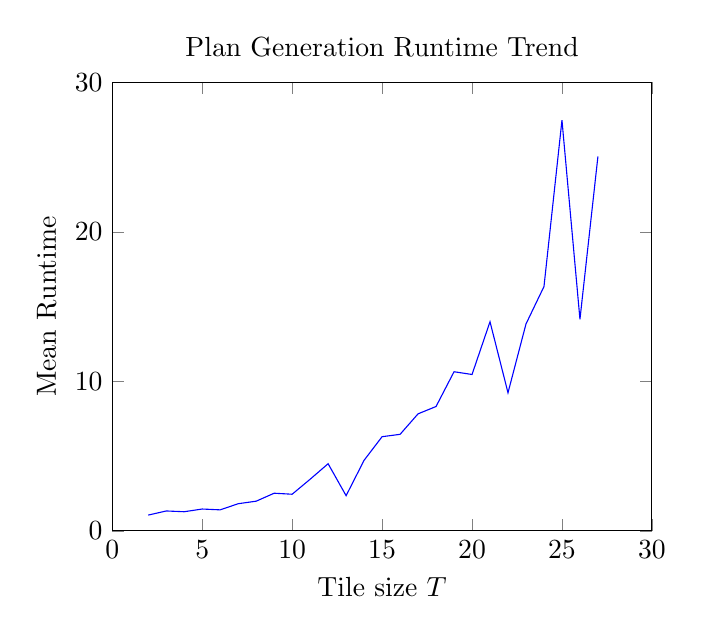
\begin{tikzpicture}
\begin{axis}[
    title={Plan Generation Runtime Trend},
    xlabel={Tile size $T$},
    ylabel={Mean Runtime},
    xmin=0, xmax=30,
    ymin=0, ymax=30,
]

\addplot[
    color=blue,
    ]
    coordinates {(2, 1.0514459609985352)
(3, 1.327857494354248)
(4, 1.2770888805389404)
(5, 1.4581902027130127)
(6, 1.402270793914795)
(7, 1.8123571872711182)
(8, 1.9829325675964355)
(9, 2.51538348197937)
(10, 2.4477152824401855)
(11, 3.4509198665618896)
(12, 4.489059686660767)
(13, 2.3502399921417236)
(14, 4.71928334236145)
(15, 6.297330141067505)
(16, 6.456403493881226)
(17, 7.827086925506592)
(18, 8.318503856658936)
(19, 10.644485712051392)
(20, 10.46013331413269)
(21, 13.989691734313965)
(22, 9.238670349121094)
(23, 13.84094762802124)
(24, 16.344945669174194)
(25, 27.47840189933777)
(26, 14.154968738555908)
(27, 25.057862758636475)};
    
\end{axis}
\end{tikzpicture}
\caption{Runtime on the generation of plans with increasing $T$}
\end{figure}

\subsection{Evaluation}
Overall, the generalised planner took exponentially more time to arrive at a solution than the classical planner where $T \geq 3$, most likely due to the lack of similarities between problems within $\mathcal{P}$. This was the case for all problems generated by any problem generator, except the problems created from a problem reduction were solved significantly faster.

\section{Comparative Analysis of Maze Problems}
This experiment involves comparing the runtime of the BFGP++ generalised planner on a fixed set of problems generated by the various problem generators mentioned within this report. For this, the tile size will remain constant at $T=5$ and each problem set $\mathcal{P}$ will contain 3 problems. An mean runtime will be taken over a set of 5 problem sets, the images of these Maze problems will be given in the Appendix. 

\subsection{Problems with No Turns}
This first set of problem sets contains Maze problems that contain no turnings that the agent has to make. This experiment aims to determine whether the absence of actions that involve re-orientating the agent will have an effect on the performance of the planner. The results generated in this experiment is given below:

\begin{table}[ht]
\centering
\begin{tabular}{|p{0.25\linewidth}|p{0.09\linewidth}|p{0.09\linewidth}|p{0.09\linewidth}|p{0.09\linewidth}|p{0.09\linewidth}|p{0.12\linewidth}|}
\hline
Problem Generator & $\mathcal{P}_1$ & $\mathcal{P}_2$ & $\mathcal{P}_3$ & $\mathcal{P}_4$ & $\mathcal{P}_5$ & Mean \\\hline
Maze & DNF & DNF & DNF & DNF & DNF & DNF
\\\hline
Directional Maze & 0.1s & 0.1s & 0.3s & 0.3s & 0.3s & 0.22s
\\\hline
Non-Directional Maze & 2.6s & 0.02s & 0.7s & 0.4s & 0.03s & 0.75s
\\\hline
\end{tabular}
\caption{Results for the "Problems with No Turns" experiment}
\end{table}

\subsubsection{Evaluation}
Surprisingly, although there were no turning actions involved, the generalised planner could not find a solution in a reasonable time frame (60s) to solve a single problem. Even more surprisingly, is that on average the Non-Directional problem generator took more that double the amount of time for the same set of problems. Excluding the outlier of 2.6s, the average would be 0.23s which is still higher than the average taken in the Directional Maze problems. This could be the case as there are multiple solutions in each method used to solve the Directional problems, due to its structure. This could lead to the planner being able to observe a variety of states which correspond to the same real-world action, simplifying the number of states required to search for a solution. 

\subsection{Identical Problems}
This second set of problem sets contains Maze problems that are identical to each other within the set. These problems can contain turns. I hypothesise that the generalised planner will be able to compute a solution almost instantly in all problem generators as all the problems share similarities. Shown below is the results of this experiment:

\begin{table}[ht]
\centering
\begin{tabular}{|p{0.25\linewidth}|p{0.09\linewidth}|p{0.09\linewidth}|p{0.09\linewidth}|p{0.09\linewidth}|p{0.09\linewidth}|p{0.12\linewidth}|}
\hline
Problem Generator & $\mathcal{P}_1$ & $\mathcal{P}_2$ & $\mathcal{P}_3$ & $\mathcal{P}_4$ & $\mathcal{P}_5$ & Mean \\\hline
Maze & 0.1s & DNF & DNF & DNF & DNF & DNF
\\\hline
Directional Maze & 0.1s & 0.3s & 0.6s & 1.4s & 1.8s & 0.84s
\\\hline
Non-Directional Maze & 0.02s & 0.03s & DNF & DNF & DNF & DNF
\\\hline
\end{tabular}
\caption{Results for the "Identical Problems" experiment}
\end{table}

\subsubsection{Evaluation}
In all cases, the generators were able to solve the identical problems containing a straight line, almost instantly. However, in cases where there was a turn the Maze generator started falling off, failing to produce a solution in a reasonable time frame. Oddly, for problem sets containing two or more turns, the planner started to fail on the Non-Directional Maze problems. Overall, the only generator that passed every test was the Directional Maze generator, which was able to handle all the problem sets.

\subsection{Analysis on the Effect of the Maze Problem Reduction}
For a set of problems that share no similarities between them, problems with the initial Maze domain were too complex for the generalised planner to solve them. As the domain only contains a single action after the reduction, the generalised planner only focuses on where to put a move action rather than having to orientate the agent. This takes up significantly less program lines in the resultant generalised solution as well. Furthermore, the generalised planner can generate plans at a similar rate regardless if there is a turning in the Maze. To put it into perspective, the problems in set in Figure 3.15 would take roughly the same amount of time if they are generated by either generator. If any problem in that set contained a turning, it would take exponentially more time for the planner to solve it, if that problem was generated on the initial Maze domain. In either the Directional or Non-Directional problems, there would be almost no change.\\\\
Overall, in all experiments, plans generated on problems created in the Directional Maze problems, yield the best results. It was able to handle instances where there were little similarities, as well as being able to handle the orientation of the agent in problems that involved turns.

\section{Aside: Efficiency of Generalised Solutions}
This aside experiment will explore a point of interest that came up during the development of this project. Although this is proven incorrect later, it still provides some insight to those interested in the field. This experiment involves measuring the efficiency of solutions generated by a generalised plan $\Pi$. The measure of \textit{inefficiency} $\overline{E}$ of a generalised solution is given by the cost of the classical plan generated through classical planning divided by the cost of the classical plan generated through generalised planning.

\subsection{Hypothesis}
\textit{There is a relationship between the efficiency of a solution and the number of program lines available to the generalised planner.} When the planner is limited to small number of program lines $PL \leq 15$, the solutions tend to be more inefficient as seen in Figure 3.16. If a classical planner can solve the same problem in 3 lines, the inefficiency score of generalised solution given in Figure 3.16 is $\frac{8}{3} = 2.\dot{6}$. In this report, a plan is \textit{efficient enough} if $\overline{E} \leq 1.5$. Figure 4.3 shows the relationship between the mean inefficiency score $\frac{\Sigma\overline{E}}{|\mathcal{P}|}$, over the set of problems $\mathcal{P}$, and the number of program lines $10 \leq PL \leq 50$ in the synthesis of generalised plans for the following set of problems shown in Figure 4.2. This experiment uses the Directional problem generator to generate the three problems.

\begin{figure}[h!]
    \centering
    \includegraphics[width=0.75\textwidth]{images/genplanexperiment.png}
    \caption{Maze problems evaluated in the "Efficiency" experiment}
\end{figure}

\begin{figure}[h!]
    \centering
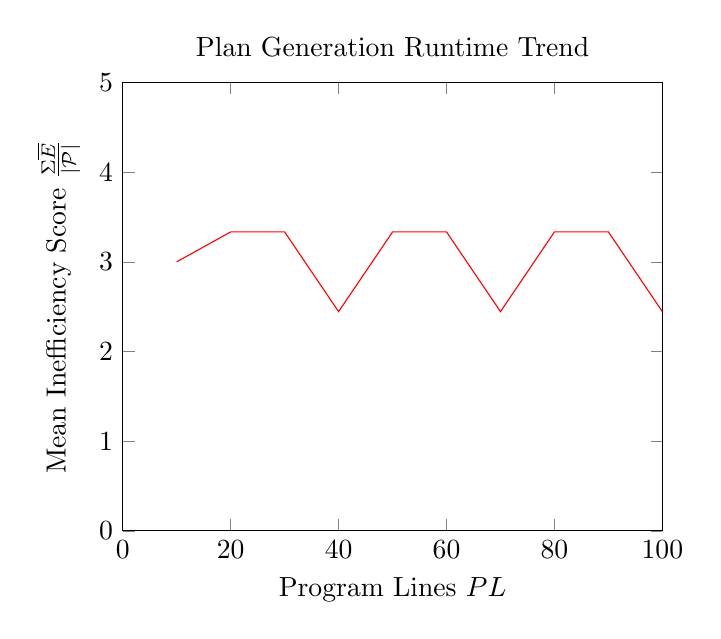
\begin{tikzpicture}
\begin{axis}[
    title={Plan Generation Runtime Trend},
    xlabel={Program Lines $PL$},
    ylabel={Mean Inefficiency Score $\frac{\Sigma\overline{E}}{|\mathcal{P}|}$},
    xmin=0, xmax=100,
    ymin=0, ymax=5,
]

\addplot[
    color=red,
    ]
    coordinates {(10, 3.0)(20, 3.3333333333333335)(30, 3.3333333333333335)(40, 2.4444444444444446)(50, 3.3333333333333335)(60, 3.3333333333333335)(70, 2.4444444444444446)(80, 3.3333333333333335)(90, 3.3333333333333335)(100, 2.4444444444444446)};
    
\end{axis}
\end{tikzpicture}
\caption{Plot of Mean Inefficiency Scores $T$}
\end{figure}

\subsection{Evaluation}
Overall, Figure 4.3 shows that there is \textit{not} a relationship between the program lines and plan efficiency, disproving the hypothesis. The optimal amount of plan lines for this problem is at 40, 70 or 100 where the mean inefficiency score is at its lowest. From this graph, at no point was a plan of any length classified as efficient enough. This could suggest that either the boundary for efficient generalised solutions is too high or that the planner cannot generate a plan efficient enough for this set of problems. This experiment can be carried out at a larger scale, taking into account the effect of a variety of problems, in future work. This evaluation was done due to the interest of understanding the consequence of modifying program lines in the synthesis of generalised plans.

\chapter{Summary and Conclusions}
\section{Summary}
In this project, I have successfully investigated the applicability of generalised planning in complex path finding games, as well as created a tool in which planning instances can be created and customised. In this, I explored a variety of games: Maze and Snake. When creating these, I realised that they were far too complex for the generalised planner to find solutions, and hence performed a problem reduction. This led to a significant improvement in the synthesis of generalised plans. In addition to the creation of problems, I also evaluated the effect of larger environments, where the agent must travel further to reach a goal. In this, I discovered that the generalised planner did not perform as well as the classical planner for very large environments. In a third and final experiment, I also explored the effect of increasing the length of the algorithm created in a generalised plan, to determine whether this would generate better classical plans. This did not meet expectations, as there was no correlation between the length of the program and cost of the classical plans. To end this summary, I also gained a wide variety of knowledge on knowledge-based agents as well as gaining a deeper insight into Automated Planning as a field.

\newpage
\section{Achievements}
The initial aims and objective have been met as well as exceeded with the introduction of problem reductions. The below table lists the objectives and how they were met in this project.

\begin{table}[ht]
\centering
\begin{tabular}{|p{0.473\linewidth}|p{0.473\linewidth}|}
\hline
Objective & How it was achieved \\\hline
Explore state-of-the-art planners used in Automated Planning in recent years & I have researched into the history of planners and knowledge-based agents, and utilised two planners that are currently well known and appreciated for being the best in the field. Furthermore, I have gained more knowledge on first-order-logic which has its importance outside of AI. \\\hline
Model path finding problems (Maze and Snake) as planning problems & I was able to model both the Maze and Snake problems, as well as providing a problem reduction on the Maze problems that yield more optimal results.
\\\hline
Create easy-to-understand visuals that displays generated path finding problems & I created an interactive display for the Maze generator, where the user can create custom Maze problems. However I was not able to do this for the Snake problems.\\\hline
Perform analysis on the performance of generalised planning on the created path finding problem instances & As described in the Experiments section, I was able to evaluate a variety of cases in which the generalised planner performed well and where it has its limitations.
\\\hline
Compare the plans generated by classical plans and generalised plans & Finally, I was able to measure the generalised plan's performance against a set of classical plans, shown in the Experiments section.
\\\hline
\end{tabular}
\caption{Goals Achieved}
\end{table}
\noindent Overall, I am proud of this project, as it was able to meet all the criteria I set. Furthermore, the knowledge gained from this is invaluable as the field of AI is ever growing.

\section{Critical Reflections}
Although all the criteria in this project's objectives was met, there are several areas for improvement. Currently the generation of Mazes still have some bugs in them, although usable, sometimes when setting the start and goal nodes, if the user wants to change the start node, sometimes it causes the program to crash. Furthermore, I would've liked to implement a manual generation option for the Snake games, had more time been available.  A final point to reflect on is that, if I were to re-do this project, I would plan the structure a lot earlier before developing. By following a strict iterative approach after having programmed for a couple months set me moderately far behind, potentially reducing the scale of this project. A better plan would have involved thinking about the core of the program first, which was the problem generator. Despite this, I am satisfied that the generalised planner is able to solve the problems I have created, as well as the optimisations made within the Maze domain, as this is the main focus of the investigation of this project.

\section{Future Work}
Following the research done by this project, in future works, I would like to extend the problem reduction to a variety of different domain models, potentially devising a solution that can be applied to any domain model. In terms of the visual aspects of this project, I would like to develop a more sophisticated user interface that allows the user to create new problems as well as being able to view the plans in real time. Furthermore, I would like to implement other games in the Blockly series such as the Bird game that involves the agent moving a fixed distance over a specific orientation. Overall, the most of the proposed future developments would involve making the project look better, which is a testament to the goals achieved in the development of this project.

\bibliographystyle{plain}
\bibliography{refs}

\appendix
\chapter{Scripts and Images}
\section{CLI Flags}
\begin{figure}[h!]
\centering
\begin{BVerbatim}
PDDL Path Solver

options:
  -h, --help            show this help message and exit
  -d {blockly_maze,directional_maze,non_directional_maze,snake}, 
  --domain {blockly_maze,directional_maze,non_directional_maze,snake}
  -r DISPLAY_PROBLEMS, --display_problems DISPLAY_PROBLEMS
  -t {each,all}, --solution_type {each,all}
  -a, --auto
  -p PROBLEM_COUNT, --problem_count PROBLEM_COUNT
  -l PROGRAM_LINES, --program_lines PROGRAM_LINES
  -s TILE_SIZE, --tile_size TILE_SIZE
  -i IMAGE_DIRECTORY, --image_directory IMAGE_DIRECTORY
  -j PLAN_DIRECTORY, --plan_directory PLAN_DIRECTORY
  -k PROBLEM_DIRECTORY, --problem_directory PROBLEM_DIRECTORY
  -c APPLE_COUNT, --apple_count APPLE_COUNT
\end{BVerbatim}
\caption{Help text describing the usage of the program}
\end{figure}

\hfill
\section{Unified Planning Examples}
\subsection{Directional Maze Problem}
\newpage

\begin{figure}[h!]
\centering
\begin{BVerbatim}
problem name = reduced_maze0

types = [position]

fluents = [
  bool path[a=position, b=position]
  bool at[x=position]
]

actions = [
  action move(position x, position xn) {
    preconditions = [
      (at(x) and path(x, xn))
    ]
    effects = [
      at(xn) := true
      at(x) := false
    ]
  }
]

objects = [
  position: [start, goal, u0, ..., l14]
]

initial fluents default = [
  bool path[a=position, b=position] := false
  bool at[x=position] := false
]

initial values = [
  at(start) := true
  path(start, u0) := true
  ...
  path(r6, goal) := true
]

goals = [
  at(goal)
]
\end{BVerbatim}
\caption{Example Unified Planning instance}
\end{figure}

\newpage \hfill
\section{Images Used in Experiments}
\subsection{Problems with No Turns}

\begin{figure}[h!]
\centering
\includegraphics[width=0.7\textwidth]{experiment_images/p1.png}
\includegraphics[width=0.7\textwidth]{experiment_images/p2.png}
\includegraphics[width=0.7\textwidth]{experiment_images/p3.png}
\includegraphics[width=0.7\textwidth]{experiment_images/p4.png}
\includegraphics[width=0.7\textwidth]{experiment_images/p5.png}
\caption{Experiment images for "Problems with No Turns"}
\end{figure}

\newpage \hfill
\subsection{Identical Problems}

\begin{figure}[h!]
\centering
\includegraphics[width=0.7\textwidth]{experiment_images/i1.png}
\includegraphics[width=0.7\textwidth]{experiment_images/i2.png}
\includegraphics[width=0.7\textwidth]{experiment_images/i3.png}
\includegraphics[width=0.7\textwidth]{experiment_images/i4.png}
\includegraphics[width=0.7\textwidth]{experiment_images/i5.png}
\caption{Experiment images for "Identical Problems"}
\end{figure}

\end{document}
https://www.sciencedirect.com/science/article/pii/S000437022400033X